% C1、C2 与阴影区域的示意重绘；图中取 a=1 仅为排布，非题设附加条件。
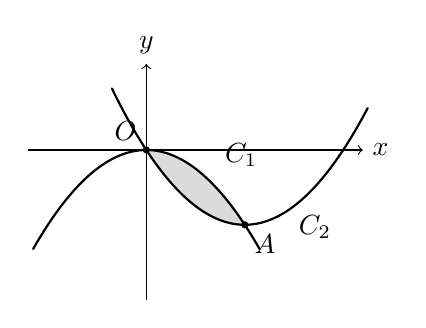
\begin{tikzpicture}[x=1.25cm,y=0.95cm,line cap=round,line join=round]
  \fill[gray!28] (0,0)
    -- plot[domain=0:1,samples=60] (\x,{ -\x*\x })
    -- plot[domain=1:0,samples=60] (\x,{ \x*\x-2*\x }) -- cycle;
  \draw[->] (-1.2,0)--(2.2,0) node[right] {$x$};
  \draw[->] (0,-2.0)--(0,1.15) node[above] {$y$};
  \draw[thick,domain=-1.15:1.15,samples=80] plot (\x,{ -\x*\x });
  \draw[thick,domain=-0.35:2.25,samples=80] plot (\x,{ \x*\x-2*\x });
  \fill (0,0) circle (1.3pt) node[above left] {$O$};
  \fill (1,-1) circle (1.3pt) node[below right] {$A$};
  \node[above right] at (0.7,-0.35) {$C_1$};
  \node[below right] at (1.45,-0.75) {$C_2$};
\end{tikzpicture}
